\documentclass[9pt,table]{beamer} % options fleqn

\usepackage{/home/paul/Workspace/build/macros}


\usetheme[titleformat frame = smallcaps]{metropolis}
%\usepackage{FiraSans}
\usepackage{FiraMono}

\metroset{sectionpage=none}

%\usepackage[T1]{fontenc}


%\setbeamersize{text margin left=5mm,text margin right=5mm} 
%\setbeamersize{text margin left=9mm,text margin right=3mm} 

\setbeamertemplate{section in toc}[sections numbered]

% algorithms
\usepackage[ruled,linesnumbered]{algorithm2e}
\SetKwInput{KwInput}{Input}
\SetKwInput{KwOutput}{Output}

% typography
\usepackage{soul}

\usepackage{caption}

\usepackage{varwidth}

\usepackage{dsfont}

\usepackage[gen]{eurosym}

% figures
\usepackage{svg}
%\svgpath{{figs/}}

\usepackage{algorithmic}

% drawings
\usepackage{tikz}
\usetikzlibrary{shapes,shapes.misc,shapes.geometric}
\usetikzlibrary{positioning,fit,backgrounds}
\usetikzlibrary{trees,matrix}
\usetikzlibrary{decorations.pathreplacing,calligraphy}
%
\tikzset{cross/.style={cross out, draw=red, minimum size=3pt, line width=0.25mm, inner sep=0pt, outer sep=0pt}, cross/.default={1pt}}
%
\usepackage[skins,theorems]{tcolorbox}
\tcbset{highlight math style={colback=mLightBrown!20,colframe=black!2,sharp corners},bottom=2pt,top=2pt}
\tcbset{left skip={-.01\linewidth}, colback=mLightBrown!20,colframe=black!2,sharp corners,left=0pt,right=0pt}
%
\newcommand{\point}[1]{\textbf{\textcolor{mDarkTeal}{#1}}\quad}
%
%\definecolor{cobalt}{HTML}{0047AB}
\definecolor{aqua}{HTML}{00FFFF}
\newcommand{\kw}[1]{\textbf{\alert{#1}}}
\newcommand{\invsible}[1]{\textcolor{black!2}{#1}}
%
\definecolor{myteal}{rgb}{0.21, 0.46, 0.53}

\usepackage[position=bottom]{subfig}

\usepackage{tabularx}
\usepackage{booktabs}% http://ctan.org/pkg/booktabs
\newcommand{\tabitem}{\llap{\tiny$\blacksquare$}~~}



% specific comands
% **********************
\newcommand{\mlprod}[4]{[\![#1;\, #2, #3, #4]\!]}
\newcommand{\cpd}[3]{[\![#1, #2, #3]\!]}

% TikZ styles for drawing
\tikzstyle{block} = [draw,rectangle,thick,minimum height=2em,minimum width=2em]
\tikzstyle{sum} = [draw,circle,inner sep=0mm,minimum size=2mm]
\tikzstyle{connector} = [->,thick]
\tikzstyle{line} = [thick]
\tikzstyle{branch} = [circle,inner sep=0pt,minimum size=1mm,fill=black,draw=black]
\tikzstyle{guide} = []

\def\R{\mathbfhbb{R}}
\def\C{\mathbfhbb{C}}
\def\H{\mathbfhbb{H}}
\def\HC{{\mathbfhbb{H}_\mathbfhbb{C}}}
\def\im{\texttt{i}}
\def\jm{\texttt{j}}
\def\km{\texttt{k}}
%\def\e{\mathbfhrm{e}}
\def\b{\mathbfhbf}
\def\cal{\mathbfhcal}

\newcommand{\bfa}{\mathbf{a}}
\newcommand{\bfb}{\mathbf{b}}
\newcommand{\bfc}{\mathbf{c}}
\newcommand{\bfd}{\mathbf{d}}
\newcommand{\bfM}{\mathbf{M}}

\newcommand{\vect}[1]{\mathbf{#1}}
\newcommand{\matr}[1]{\mathbf{#1}}

\newcommand{\Blue}[1]{\textcolor{blue}{#1}}
\newcommand{\Red}[1]{\textcolor{red}{#1}}
\newcommand{\Green}[1]{\textcolor{green}{#1}}

\newcommand{\T}{\top}

% ************************


% handling lists
\usepackage{enumitem}

\usepackage{multimedia}

\usepackage{animate}
\usepackage{pifont}% http://ctan.org/pkg/pifont
\newcommand{\cmark}{\ding{51}}%
\newcommand{\xmark}{\ding{55}}%

% tcolorbox
\usepackage[skins,theorems]{tcolorbox}
\tcbset{highlight math style={colback=mLightBrown!20,colframe=black!2,sharp corners},bottom=2pt,top=2pt}
\tcbset{left skip={-.01\linewidth}, colback=mLightBrown!20,colframe=black!2,sharp corners,left=0pt,right=0pt}


% references
\usepackage[backend=biber,style=authoryear]{biblatex}
%\usepackage[backend=biber,style=alphabetic]{biblatex}
\bibliography{/home/paul/Workspace/build/biblio}
\usepackage{bibentry}
\newcommand{\mycite}[2]{\footnotetext[#1]{\emph{\tiny{\citeauthor{#2},\,\citeyear{#2},}}\,\tiny{\citefield{#2}{title}}}}

%\renewcommand{\cite}[1]{\textcolor{myteal}{[\citeauthor{#1},\,\citeyear{#1}]}}%
%\newcommand{\mycite}[1]{\textcolor{myteal}{\cite{#1}}}%
\AtBeginEnvironment{frame}{\setcounter{footnote}{0}}

\usepackage{hyperref}


\graphicspath{{figs/}{examples/}{/home/paul/Workspace/data/standard_test_images}}




% add a sommaire
%\makeatletter
%\setbeamertemplate{headline}{%
%  \begin{beamercolorbox}[colsep=1.5pt]{upper separation line head}
%  \end{beamercolorbox}
%  \begin{beamercolorbox}{section in head/foot}
%    \vskip2pt\insertnavigation{\paperwidth}\vskip2pt
%  \end{beamercolorbox}%
%  \begin{beamercolorbox}[colsep=1.5pt]{lower separation line head}
%  \end{beamercolorbox}
%}
%\makeatother

\setbeamertemplate{theorem begin}
{%
  \inserttheoremheadfont% \bfseries
  \inserttheoremname \inserttheoremnumber
  \ifx\inserttheoremaddition\@empty\else\ (\inserttheoremaddition)\fi%
  \inserttheorempunctuation
  \normalfont
}
\setbeamertemplate{theorem end}{%
  % empty
}
\makeatother

\setbeamercolor{section in head/foot}{fg=normal text.bg, bg=structure.fg}



\title{Optimisation Numérique et Sciences des Données}
\subtitle{Sciences des données -- Décompostion tensorielles pour les tableaux de données}
\author{Paul Catala (CRAN, UL) \hfill Master Ingénierie des Systèmes Complexes}
%\date{Postdoctorant à l'université d'Osnabrück, Allemagne}
\date{paul.catala(at)univ-lorraine.fr \hfill Semestre 9 -- 2025 \\ \\ D'après un cours de D. Brie, S. Miron et K. Usevich}

\titlegraphic{
\includegraphics[width=2cm]{figures/cube}}



\begin{document}
\maketitle

\section{Tableaux multidimensionnels}

\begin{frame}[noframenumbering,plain]{Plan}
\tableofcontents[currentsection]
\end{frame}

\begin{frame}
\frametitle{Applications}

\begin{itemize}
	\item[\tiny$\blacksquare$] \alert{Apprentissage automatique}: modélisation des distributions, réseaux de neurones, clustering, graphes
	\item[\tiny$\blacksquare$] \alert{Chimiométrie}: MEEF, microscopie Raman polarisée
	\item[\tiny$\blacksquare$] \alert{Imagerie médicale}: IRM, tomographie, EEG
	\item[\tiny$\blacksquare$] \alert{Traitement d'antennes}: radar, astronomie, acoustique sous-marine, géophysique, MIMO
\end{itemize}

\begin{tcolorbox}
Les données viennent souvent sous la forme
\begin{center}
capteur $\times$ caractéristique$_1$ $\times$ $\ldots$ $\times$ caractéristique$_n$
\end{center}

Décomposition tensorielles:
\begin{itemize}
	\item[-] Compression
	\item[-] Modélisation
	\item[-] Fusion de données
	\item[-] Explicabilité (caractéristiques dominantes, détection d'anomalies, ...)
\end{itemize} 
\end{tcolorbox}
\end{frame}

\begin{frame}
\frametitle{Tableaux multidimensionnels}
\textbf{\large Fonction multivariable:}
\begin{equation*}
\begin{aligned}
%\label{}
	&\mathbf{v} = [v_1, \cdots, v_N] \\
 &x: \mathbb{R}^N \rightarrow \mathbb{R}\\
     & \mathbf{v} \mapsto x(\mathbf{v} )
\end{aligned}
\end{equation*}
\textbf{\large Cas discret} : en échantillonnant $x(\mathbf{v})$ sur une grille regulière, on obtien un \alert{tableau multidimensionnel} de valeurs

$$\mathcal{X}_{i_1 i_2 \cdots  i_N}$$

On assimile un tenseur $\mathcal{X}$ à un tableau multidimensionnel. \\
$N$ : ordre d'un tenseur (= nombre de modes)
\end{frame}






\begin{frame}\frametitle{Exemples et notation}
\begin{itemize}
\item ($N=0$) Scalaire $s$ 
\item ($N=1$) vecteur $\mathbf{v}=[v_i]$ 
\item ($N=2$) matrice $\mathbf{M}=[m_{ij}]$ 
\item ($N \ge 3$) tenseur $\mathcal{T}= [t_{ijk}]_{i,j,k=1}^{I,J,K}$, $(\mathcal{T})_{ijk}= t_{ijk}$
\[

\includegraphics[height=0.4\textwidth]{figures/Tensor}
\]
\end{itemize}
\end{frame}







\begin{frame}
\frametitle{Fibres, tranches (tenseur d'ordre 3)}
\begin{itemize}
\item Fibres:
\[
\begin{array}{ccccc}
\text{colonnes} &\qquad& \text{lignes} &\qquad& \text{tubes}\\
\Xx_{:,j,k} && \Xx_{i,:,k} &&  \Xx_{i,j,:} 
\end{array}
\]
\[

\includegraphics[height=2cm]{figures/fibers.png}
\]
\item Tranches:
\[
\begin{array}{ccccc}
\text{horizontales} & \qquad&\text{latérales} & \qquad&\text{frontales} \\
\Xx_{i,:,:} & & \Xx_{:,j,:} &&\Xx_{:,:,k} 
\end{array}
\]
\[

\includegraphics[height=2cm]{figures/slices.png}
\]
\end{itemize}
%\begin{itemize}
%\item Matrices are $2$-nd order tensors
%\item Tensors are multilinear operators
%\end{itemize}
\end{frame}

\begin{frame}\frametitle{Tenseur diagonal, tenseur symétrique}

\begin{minipage}[l][5cm][c]{0.45\textwidth}
\begin{center}
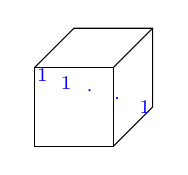
\begin{tikzpicture}\begin{scope}[scale=1]
\draw(0,0) rectangle (1,1);
\draw(0,1) -- (0.5,1.5) -- (1.5,1.5) -- (1.5,0.5) --(1,0);
\draw(1,1) -- (1.5,1.5);
\draw(0.1,0.9) node (A) {\scriptsize \textcolor{blue}{$1$}};
\draw(0.4,0.8) node (A) {\scriptsize \textcolor{blue}{$1$}};
\draw(0.7,0.7) node (A) {\scriptsize \textcolor{blue}{$\cdot$}};
\draw(1.05,0.6) node (A) {\scriptsize\textcolor{blue}{$\cdot$}};
\draw(1.4,0.5) node (A) {\scriptsize \textcolor{blue}{$1$}};
\end{scope}\end{tikzpicture}
\\[3.2ex]
Tenseur diagonal
$$
(\mathcal{X})_{ijk} \neq 0 \text{ ssi } i =j=k
$$
\end{center}
%
\end{minipage}
\begin{minipage}[l][5cm][c]{0.45\textwidth}
 \begin{center}
\[
{% !TEX root = UsevichGDRISIS2020.tex
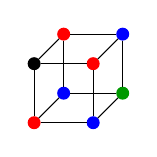
\begin{tikzpicture}
\tikzstyle{p3} = [color = green!60!black]
\tikzstyle{p2} = [color = blue]
\tikzstyle{p1} = [color = red]
\tikzstyle{p0} = [color = black]

\begin{scope}[xscale= 0.75,yscale=0.75]
\tikzstyle{dot} = [draw,circle,minimum size=1.5mm,fill,inner sep=0mm]

\draw(0,0) node[dot,p1]          (v0001) {};
\draw(1,0) node[dot,p2]          (v0011) {};
\draw(0,1) node[dot,p0]          (v0000) {};
\draw(1,1) node[dot,p1]          (v0010) {};
\draw(0.5,0.5) node[dot,p2]      (v0101) {};
\draw(1.5,0.5) node[dot,p3]      (v0111) {};
\draw(0.5,1.5) node[dot,p1]      (v0100) {};
\draw(1.5,1.5) node[dot,p2]      (v0110) {};

\draw (v0000) -- (v0010) -- (v0011) -- (v0001) -- (v0000);
\draw (v0100) -- (v0110) -- (v0111) -- (v0101) -- (v0100);
\draw (v0000) -- (v0100);
\draw (v0010) -- (v0110) ;
\draw (v0001) -- (v0101);
\draw (v0011) -- (v0111) ;

\end{scope}
\end{tikzpicture}}
\]
\\[1.8ex]
Tenseur (cubique) symétrique
$$
(\mathcal{X})_{ijk} = \mathcal{X}_{\sigma(ijk)}, \ \sigma : \text{permutation}
$$
\end{center}
\end{minipage}
\end{frame}


\begin{frame}
\frametitle{Dépliements}
\textbf{Transformation d'un tenseur en une matrice } \\[2ex]
Un tenseur $\mathcal{Y}$ peut se déplier de $N$ façons différentes : $\mathbf{Y}_{(n)}$
\[
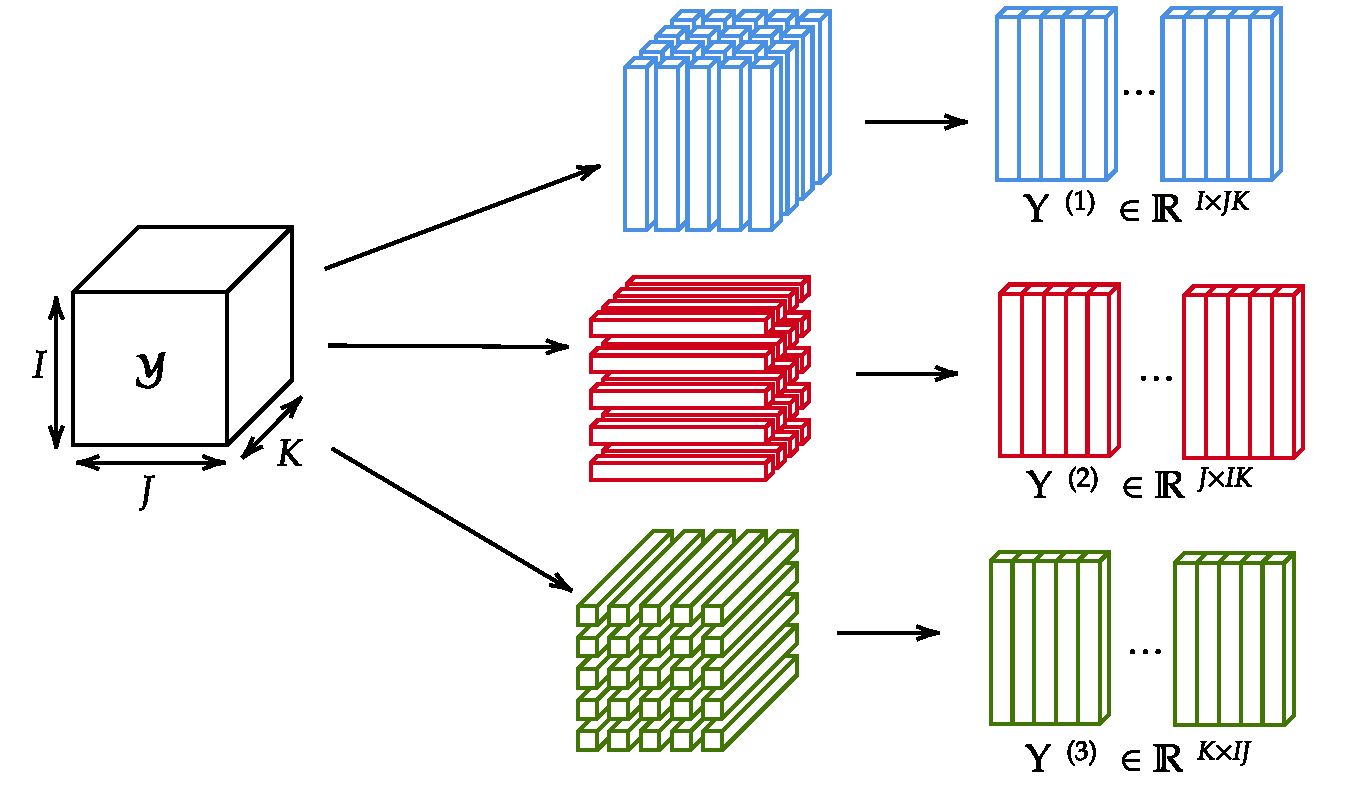
\includegraphics[height=5cm]{figures/unfold}
\]
\textbf{Transformation d'un tenseur en un vecteur}\quad
$\mathbf{y} = \text{vec}(\mathcal{Y}) \ (I J K \times 1)$

%\textbf{\color{blue} Matlab (demo 1) }
\end{frame}


\begin{frame}
\frametitle{Produits matriciels et tensoriels}
\begin{center}
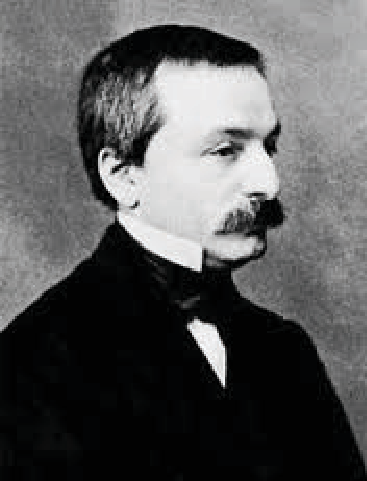
\includegraphics[width=2cm]{figures/Kron}
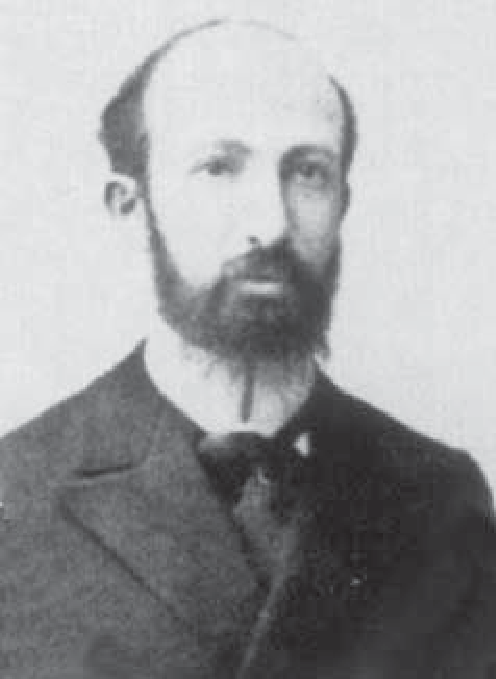
\includegraphics[width=2cm]{figures/Hadamard}
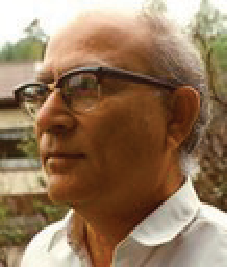
\includegraphics[width=2cm]{figures/Khatri}
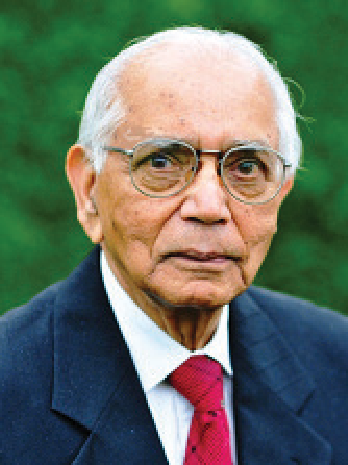
\includegraphics[width=2cm]{figures/Rao}
\end{center}
\begin{center}
Kronecker, Hadamard, Khatri-Rao
\end{center}
\end{frame}
%%%%%%%%%%%%%%%%


\begin{frame}
\frametitle{Produits matriciels et tensoriels (1)}
\textbf{Notations}
$$ \mathbf{A} = [\mathbf{a}_1 \cdots \mathbf{a}_R], \ (I \times R)
\quad
\mathbf{B} = [\mathbf{b}_1 \cdots \mathbf{b}_R], \ (J \times R)$$

\textbf{Produit de Kronnecker}

$$ \mathbf{A} \otimes  \mathbf{B}  =
 \left[   \begin{array}{ c c c}
a_{11} \mathbf{B}    &  a_{12} \mathbf{B} & \cdots    \\
a_{21} \mathbf{B}    &  a_{22}  \mathbf{B}& \cdots    \\
                                             &  \vdots                                &     
\end{array} \right]
$$

\textbf{Produit de Khatri-Rao}
 $$ \mathbf{A} \odot  \mathbf{B}  =  [\mathbf{a}_1 \otimes  \mathbf{b}_1 \cdots \mathbf{a}_R  \otimes  \mathbf{b}_R], \ (IJ \times R)$$
 
\textbf{Produit de Hadamard} (produit termes à termes)\\
$\mathbf{A}, \mathbf{B}$ matrices de même dimension $(I \times J)$ 
$$ \mathbf{A} \ast  \mathbf{B}  = [ a_{ij} b_{ij}] , (I \times J)$$
\end{frame}
%%%%%%%%%%%%%%%%%%%%%%%%%%%%%%%%%
%%%%%%%%%%%%%%%%%%%%%%%%%%%%%%%%%%

\begin{frame}
\frametitle{Produits matriciels et tensoriels (2)}

\textbf{Propriétés}\\

\[
\boxed{\text{vec}(\mathbf{A} \mathbf{X}  \mathbf{B}) = (\mathbf{B}^{T} \otimes \mathbf{A})\text{vec}(\mathbf{X})} 
\]

$$
(\mathbf{A} \otimes  \mathbf{B}  ) (\mathbf{C} \otimes  \mathbf{D}  ) = \mathbf{A}   \mathbf{C}  \otimes \mathbf{B}   \mathbf{D} 
$$

$$
(\mathbf{A} \otimes  \mathbf{B}  )^\dagger = \mathbf{A}^\dagger \otimes  \mathbf{B}^\dagger  
$$


$$
(\mathbf{A} \odot  \mathbf{B}  )\odot \mathbf{C} = \mathbf{A} \odot (\mathbf{B}  \odot \mathbf{C} ) = \mathbf{A} \odot  \mathbf{B}  \odot \mathbf{C}
$$

$$
(\mathbf{A} \odot  \mathbf{B} )^\top (\mathbf{A} \odot  \mathbf{B} ) = \mathbf{A}^\top \mathbf{A} \ast   \mathbf{B}^\top \mathbf{B}
$$

$$
(\mathbf{A} \odot  \mathbf{B} )^\dagger = (\mathbf{A}^\top \mathbf{A} \ast   \mathbf{B}^\top \mathbf{B})^\dagger (\mathbf{A} \odot  \mathbf{B} )^\top
$$



$^\top$ : transposée\\
$\dagger$: pseudoinverse

\end{frame}
%%%%%%%%%%%%%%%%%%%%%%%%%%%%%%%%%
%%%%%%%%%%%%%%%%%%%%%%%%%%%%%%%%%%

\begin{frame}
\frametitle{Produits matriciels et tensoriels (3)}
\textbf{Produit tensoriel }
$$ 
\mathbf{a} \circ \mathbf{b}, \ (I \times J),
\quad  
(\mathbf{a} \circ \mathbf{b})_{ij} = a_i  b_j\text{ \emph{i.e.} } \mathbf{a} \circ \mathbf{b} = \mathbf{a} \mathbf{b}^T, \text{ matrice de rang 1.}
$$
$$ 
\mathbf{a} \circ \mathbf{b} \circ \mathbf{c}, \ (I \times J \times K),
\quad  
(\mathbf{a} \circ \mathbf{b} \circ \mathbf{c})_{ijk}  =  a_i  b_j c_k\text{ \emph{i.e.}  tenseur de rang 1.}
$$

\textbf{Produit n-mode}
$$\mathbf{A}: \ (J \times I_n), \quad \mathcal{X}: \  (I_1 \times I_2  \cdots \times I_N )$$
$$ \mathcal{X} \times_n A : \  (I_1 \times  \cdots \times I_{n-1} \times J \times I_{n+1} \dots \times I_N )$$
$$
(\mathcal{X} \times_n A )_{i_1\cdots i_{n-1} j i_{n+1}\cdots i_{N}}= \sum_{i_n = 1}^{I_1} x_{i_1 \cdots i_{N}} a_{j i_{n}}
$$

%\textbf{\color{blue} Matlab (demo 2) }
\end{frame}
%2%%%%%%%%%%%%%%%%%%%%%%%%%%%%%%%%%%%%%%%%%%%%%%%%%%%%%%%%%%%%%%%%%%%%%%%%%%%%%%%%%%%%%%%

\section{Décompositions tensorielles}


\begin{frame}[noframenumbering,plain]{Plan}
\tableofcontents[currentsection]
\end{frame}

\begin{frame}
\frametitle{Décompositions tensorielles}
\begin{center}
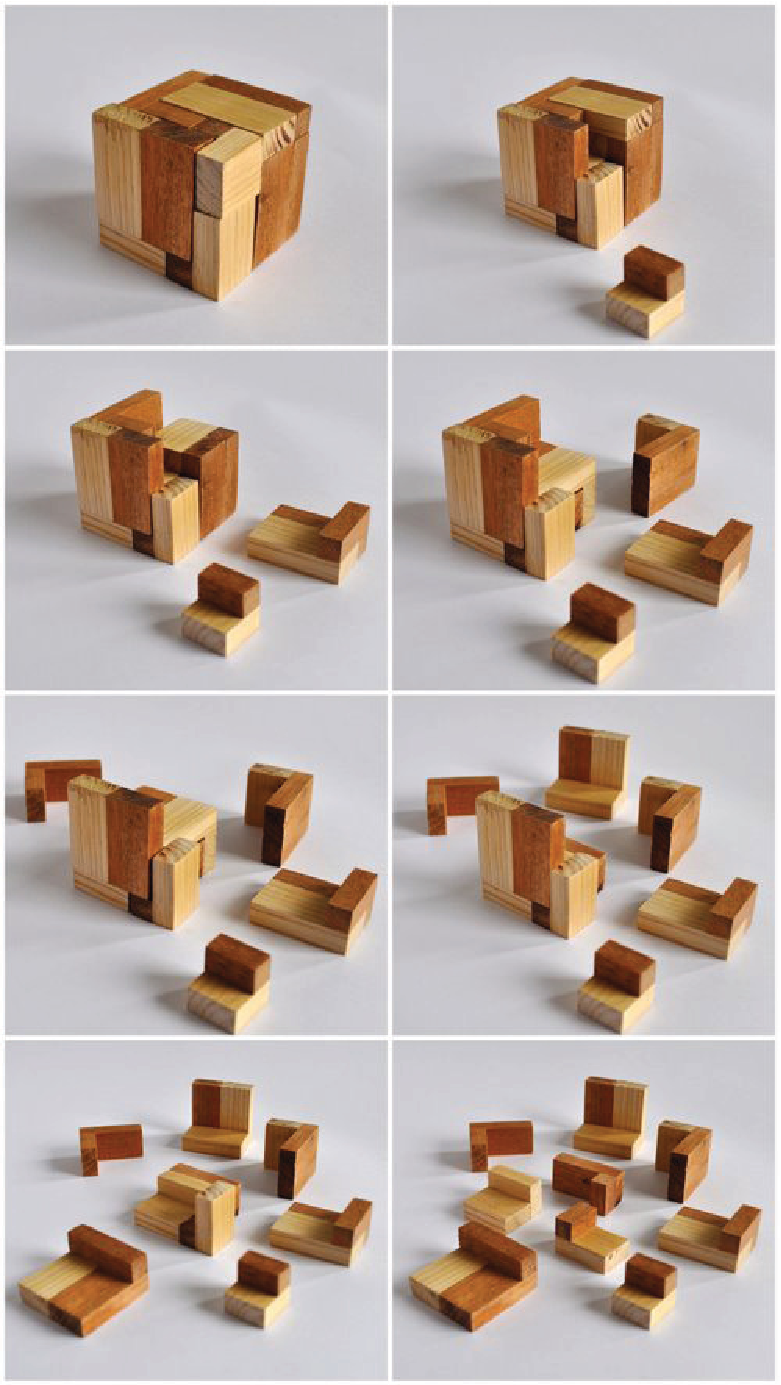
\includegraphics[width=4cm]{figures/cube_decompose}
\end{center}
\end{frame}


\begin{frame}
\frametitle{Rappel : rang matriciel}
\[
\mathbf{X} \in \mathbb{R}^{I \times J}, \quad \mathbf{X} = \sum_{r=1}^R  \mathbf{a}_{r} \mathbf{b}_{r}^T = \mathbf{A} \mathbf{B}^T
\]
\[
\raisebox{-0.35\height}{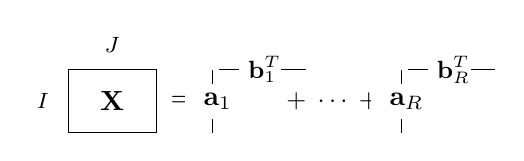
\begin{tikzpicture}[scale=0.8]
\draw(0,0.5) node (A) {$\mathbf{X}$};
\draw(-1.1,0.5) node (eq) {\footnotesize ${I}$};
\draw(0,1.4) node (eq) {\footnotesize ${J}$};
\draw(-0.7,0) rectangle (0.7,1);
\draw(1.1,0.5) node (eq) {${=}$};
\draw(1.6,0) -- (1.6,1);
\draw(1.6,0.5) node[fill=white] (a1) {{ $\bfa_1$}};
\draw(1.7,1) -- (3.08,1);
\draw(2.35,1) node[fill=white] (b1) {{\small $\bfb_1^{T}\!\!$}};
\draw(3.5,0.5) node () {{\small $+\; \cdots\;+$}};
\draw(4.6,0) -- (4.6,1);
\draw(4.6,0.5) node[fill=white] (a1) {{ $\bfa_R$}};
\draw(4.7,1) -- (6.08,1);
\draw(5.35,1) node[fill=white] (b1) {{\small $\bfb_R^{T}\!\!$}};
\end{tikzpicture}}
\raisebox{-0.35\height}{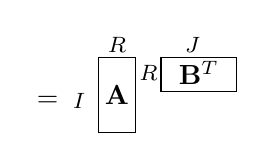
\begin{tikzpicture}[scale=0.8]
%\draw(0,0.5) node (A) {$\mathbf{X}$};
%\draw(-1.1,0.5) node (eq) {\footnotesize ${m}$};
%\draw(0,1.4) node (eq) {\footnotesize ${n}$};
%\draw(-0.8,0) rectangle (0.8,1.2);
\draw(1.2,0.5) node (eq) {$=$};

\draw(1.7,0.5) node (eq) {\footnotesize ${I}$};

\draw(2,0) rectangle (2.6,1.2); %node {A};
\draw(2.3,0.6) node (A) {$\mathbf{A}$};

\draw(2.3,1.4) node (eq) {\footnotesize ${R}$};
%\draw(5,0.5) node (eq) {\footnotesize$\quad+\,\cdots\,+\quad$};
\draw(3.5,1.4) node (eq) {\footnotesize ${J}$};

\draw(3,0.65) rectangle (4.2,1.2); %node {A};
\draw(2.8,0.95) node (eq) {\footnotesize ${R}$};
\draw(3.6,0.95) node (A) {$\mathbf{B}^{T}$};
\end{tikzpicture}}
\]

\textbf{Rang d'une matrice} : 
\begin{itemize}
\item[1.] nombre minimal de matrices de rang 1 permettant de représenter $\mathbf{X}$
\item[2.] taille minimale de la factorisation $\mathbf{A} \mathbf{B}^T $
\end{itemize}

%No
%$\Rightarrow$ \textbf{Approximation de rang faible}\\[2ex]
%\textbf{Indéterminations} : ordre, échelle, rotation
%\begin{equation*} 
%\mathbf{A} \mathbf{B}^T = (\mathbf{A} \mathbf{T}) ( \mathbf{T}^{-1}\mathbf{B}^T)  
%= \tilde{\mathbf{A}} \tilde{\mathbf{B}}^T 
%\end{equation*}
 \textbf{Contraintes} d'orthogonalité: SVD \quad $\mathbf{X} = \mathbf{U} \mathbf{\Sigma}\mathbf{V}^{T}$
\\[2ex]


\begin{tcolorbox}
\textbf{Extension de la SVD} aux tenseurs depend de la définition du rang :
\begin{itemize}
\item[1.] Décomposition CP (canonique polyadique)
\item[2.] Décomposition Tucker: HOSVD (Higher order SVD)
\end{itemize}
\end{tcolorbox}

\end{frame}


\begin{frame}
\frametitle{Décomposition de Tucker d'un tenseur d'ordre 3}
\begin{center}
$[$Tucker, 1966$]$, $[$De Lathauwer 1997$]$\\[2ex]
\end{center}
$$(\mathcal{Y} )_{ijk}= \sum_{p=1}^{R_1} \sum_{q=1}^{R_2} \sum_{r=1}^{R_3} g_{pqr} u_{ip} v_{jq} w_{kr} $$
$$\mathcal{Y} = \sum_{p=1}^{R_1} \sum_{q=1}^{R_2} \sum_{r=1}^{R_3} g_{pqr} \mathbf{u}_{p} \circ \mathbf{v}_{q}  \circ \mathbf{w}_{r} $$

$$\mathcal{Y} = \mathcal{G} \times_1 \mathbf{U}  \times_2 \mathbf{V} \times_3 \mathbf{W} = [\![ \mathcal{G}, \mathbf{U}, \mathbf{V}, \mathbf{W} ]\!]$$
\[
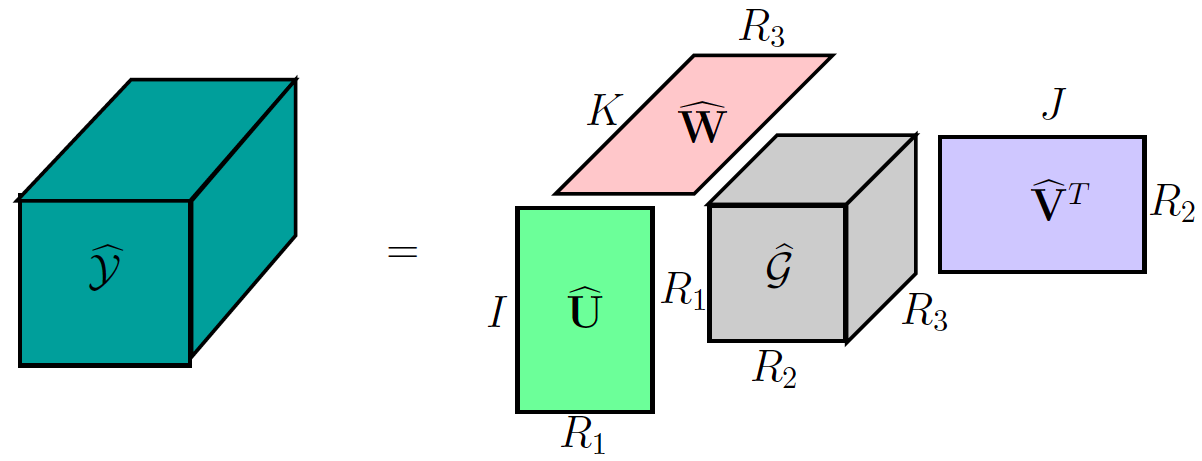
\includegraphics[height=2.5cm]{figures/tucker_exact}
\]
\begin{itemize}
\item  $\mathcal{G}$ --- tenseur coeur
\item $\mathbf{U}$, $\mathbf{V}$, $\mathbf{W}$ --- matrices facteurs
\end{itemize}
\end{frame}


\begin{frame}
\frametitle{Décomposition de Tucker d'un tenseur d'ordre N}
$$\mathcal{X} = \mathcal{G} \times_1 \mathbf{A}^{(1)}  \times_2 \mathbf{A}^{(N)}  \cdots \times_N \mathbf{A}^{(N)}  = [\![ \mathcal{G}, \mathbf{A}^{(1)} , \cdots, \mathbf{A}^{(N)}  ]\!] $$
\\[4ex]
\textbf{ Non unicité de la décomposition de Tucker}\\
$$\mathcal{X} = [\![ \mathcal{G} \times_1 \mathbf{T}_1  \times_2 \mathbf{T}_2 \times_3 \mathbf{T}_3, \mathbf{A}\mathbf{T}_1^{-1}, \mathbf{B}\mathbf{T}_2^{-1}, \mathbf{C} \mathbf{T}_3^{-1}]\!] $$
%
Contraintes : Orthogonalité des modes et du tenseur coeur 
%
$$\mathcal{X} =  [\![ \mathcal{G}, \mathbf{U}^{(1)} , \cdots, \mathbf{U}^{(N)}  ]\!] $$
\\[4ex]

\begin{tcolorbox}
\textbf{n-rank} : rang colonne du tenseur déplié selon le mode $n$ : $R_n = \text{rank}(\mathbf{X}_{(n)})$
\\[2ex]
$\Rightarrow$  \textbf{rang multilinéaire} du tenseur: $(R_1,R_2,\ldots,R_N)$
\end{tcolorbox}
\end{frame}
%procedure HOSVD(X,R1,R2, . . . , RN ) 
%for n = 1,...,N do
%A(n) ? Rn leading left singular vectors of X(n) 
%end for
%G?X×1A(1)T×2A(2)T···×N A(N)T
%return G,A(1),A(2),...,A(N) end procedure

\begin{frame}\frametitle{Algorithme HOSVD}


\scalebox{.91}{ 
\hspace*{1cm}
\begin{algorithm*}[H]
 %\caption{\label{algo}CP-ALS(X,R)}
 \KwData{ Data $\mathcal{X}$, rank-$(R_1, \cdots R_N)$ }
%\\[2ex]
 \For{$n = 1, \cdots, N$}{
   	$[\mathbf{U}_n, \bm{\Lambda}, \mathbf{V}_n] = \text{svd}(\mathbf{X}_{(n)}, R_n)$
 }
 $\mathcal{G} = \mathcal{X} \times_1 \mathbf{U}_1^\top \cdots \times_N \mathbf{U}_N^\top$\\[2ex]
 \KwResult{$\mathcal{G}, \ \mathbf{U}_1 \cdots \mathbf{U}_N$}
\end{algorithm*}
}

\textbf{Très proche d'une meilleure approximation de rang-$(R_1, \cdots R_N)$}

[De Lathauwer 1997]
\end{frame}

\begin{frame}
\frametitle{Décomposition CP d'un tenseur d'ordre 3}

CP (canonique polyadique) : Candecomp/PARAFAC
[Hitchkock, 1927] [Harshman, 1970-1972], [Carroll - Chang, 1970]

\[
\Xx = \sum\limits_{r=1}^{R} \bfa_r \circ \bfb_r \circ \bfc_r, 
\quad 
\raisebox{-0.3\height}{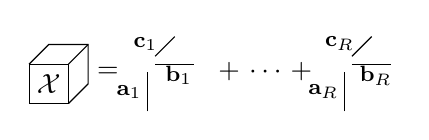
\begin{tikzpicture}
\begin{scope}[scale= 0.5]
\draw(0.5,0.5) node (A) {$\mathcal{X}$};
\draw(0,0) rectangle (1,1);
\draw(0,1) -- (0.5,1.5) -- (1.5,1.5) -- (1.5,0.5) --(1,0);
\draw(1,1) -- (1.5,1.5);

\draw(2,0.8) node (eq) {$=$};
\draw(6,0.8) node (eq) {$\quad+\,\cdots\,+\quad$};
\end{scope}

\begin{scope}[scale= 0.5,xshift=1cm]
\draw(2,-0.2) -- (2,0.8);
\draw(2.1,0.3) node[anchor=east] (s21) {\small {\footnotesize$\bfa_1$}};
\draw(2.2,1) -- (3.2,1);
\draw(2.8,1.2) node[anchor=north] (s22) {\small {\footnotesize$\bfb_1$}};
\draw(2.2,1.2) -- (2.7,1.7);
\draw(2.5,1.1) node[anchor=south east] (s23) {\small{\footnotesize$\bfc_1$}};
\end{scope}

\begin{scope}[scale= 0.5,xshift=6cm]
\draw(2,-0.2) -- (2,0.8);
\draw(2.1,0.3) node[anchor=east] (s21) {\small {\footnotesize$\bfa_R$}};
\draw(2.2,1) -- (3.2,1);
\draw(2.8,1.2) node[anchor=north] (s22) {\small {\footnotesize$\bfb_R$}};
\draw(2.2,1.2) -- (2.7,1.7);
\draw(2.5,1.1) node[anchor=south east] (s23) {\small {\footnotesize$\bfc_R$}};
%\draw(1.9,1) node (g1) {\textcolor{red}{\small $c_r$}};
\end{scope}
\end{tikzpicture}}
\]

\begin{tcolorbox}[width=\textwidth]
\textbf{rang tensoriel}  $\eqdef$ nombre minimal $R$ de tenseurs de rang 1 nécessaire pour représenter 

\hfill $\mathcal{X}$.
\end{tcolorbox}
 
  
 \vspace{2em}
 
Notation:  $\mathcal{X} = \cpd{\matr{A}}{\matr{B}}{\matr{C}}$, avec des \emph{matrices facteurs}

$\matr{A} = \begin{bmatrix}\vect{a}_1 & \cdots & \vect{a}_R \end{bmatrix}$, $\matr{B} = \begin{bmatrix}\vect{b}_1 & \cdots & \vect{b}_R \end{bmatrix}$, $\matr{C} = \begin{bmatrix}\vect{c}_1 & \cdots & \vect{c}_R \end{bmatrix}$ 
\vspace*{1cm}
\end{frame}


\begin{frame}
\frametitle{Décomposition CP (ordre 3) : écriture par tranche}

\[
\begin{array}{c@{}l}
&\mathcal{X}_{:,:,k} = \mathbf{A} \text{diag}(C_{k,:}) \mathbf{B}^{T}\\
 & 
\raisebox{-0.35\height}{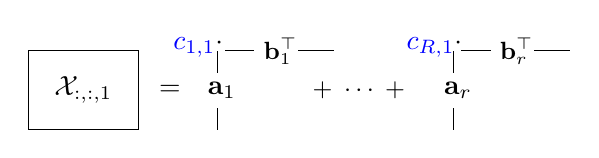
\begin{tikzpicture}
\draw(0,0.5) node (A) {$\mathcal{X}_{:,:,1}$};
\draw(-0.7,0) rectangle (0.7,1);
\draw(1.1,0.5) node (eq) {${=}$};
\draw(1.7,0) -- (1.7,1);
\draw(1.7,0.5) node[fill=white] (a1) {{ $\bfa_1$}};
\draw(1.8,1) -- (3.18,1);
\draw(2.45,1) node[fill=white] (b1) {{\small $\bfb_1^{\top}\!\!$}};
\draw(3.5,0.5) node () {{\small $+\; \cdots\;+$}};
\draw(4.7,0) -- (4.7,1);
\draw(4.7,0.5) node[fill=white] (a1) {{ $\bfa_r$}};
\draw(4.8,1) -- (6.18,1);
\draw(5.45,1) node[fill=white] (b1) {{\small $\bfb_r^{\top}\!\!$}};

\draw(1.4,1.05) node (eq) {{ $\textcolor{blue}{c_{1,1}}\cdot$}};
\draw(4.4,1.05) node (eq) {{ $\textcolor{blue}{c_{R,1}}\cdot$}};
\end{tikzpicture}} \\
 & \qquad{\vdots} \\
& 
{\raisebox{-0.35\height}{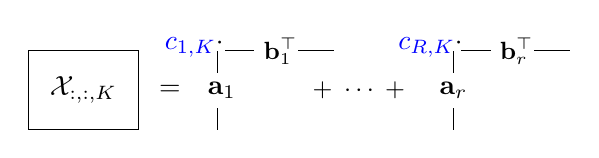
\begin{tikzpicture}
\draw(0,0.5) node (A) {$\mathcal{X}_{:,:,K}$};
\draw(-0.7,0) rectangle (0.7,1);
\draw(1.1,0.5) node (eq) {${=}$};
\draw(1.7,0) -- (1.7,1);
\draw(1.7,0.5) node[fill=white] (a1) {{ $\bfa_1$}};
\draw(1.8,1) -- (3.18,1);
\draw(2.45,1) node[fill=white] (b1) {{\small $\bfb_1^{\T}\!\!$}};
\draw(3.5,0.5) node () {{\small $+\; \cdots\;+$}};
\draw(4.7,0) -- (4.7,1);
\draw(4.7,0.5) node[fill=white] (a1) {{$\bfa_r$}};
\draw(4.8,1) -- (6.18,1);
\draw(5.45,1) node[fill=white] (b1) {{\small $\bfb_r^{\T}\!\!$}};
\draw(1.35,1.05) node (eq) {{ $\textcolor{blue}{c_{1,K}}\cdot$}};
\draw(4.35,1.05) node (eq) {{ $\textcolor{blue}{c_{R,K}}\cdot$}};
\end{tikzpicture}}} \\
& \qquad\qquad\;\; {\Updownarrow} \\
& \Xx = \sum\limits_{r=1}^{R} \bfa_r \circ \bfb_r \circ \bfc_r = \cpd{\matr{A}}{\matr{B}}{\matr{C}}
\\
\end{array}
\]
\end{frame}


\begin{frame}
\frametitle{Décomposition CP d'un tenseur d'ordre N}
%\end{center}
\begin{gather*} 
\mathcal{X} = \sum_{r=1}^R  \mathbf{a}_{r}^{(1)} \circ \cdots \circ \mathbf{a}_{r}^{(N)}=[\![ \mathbf{A}^{(1)}, \cdots , \mathbf{A}^{(N)}]\!] 
\end{gather*}
%\\[2ex]
\textbf{Ecriture alternative par dépliage}: 
\[
\mathbf{X}_{(1)} =\mathbf{A}^{(1)}  (\mathbf{A}^{(N)} \odot \cdots \odot \mathbf{A}^{(2)})^T, \ {(I_1 \times I_2 \cdots I_N)}
\]


Cas $N=3$: $\mathbf{X}_{(1)} =\mathbf{A}   (\mathbf{C} \odot \mathbf{B})^T, \ {(I \times JK)}$
\end{frame}

\begin{frame}\frametitle{Rang tensoriel}

\textbf{Rang du tenseur} : nombre minimal de tenseur de rang 1 nécessaire pour représenter 
$\mathcal{X}$.
Définition analogue au cas matriciel ... mais le rang tensoriel a des propriétés très différentes !
\\[1ex]
\begin{itemize}[label=\tiny$\blacksquare$]
\item Le rang d'un tenseur peut être différent si on considère une décomposition sur $\mathbb{R}$ ou $\mathbb{C}$
\item \alert{Rang maximal}
\[
\text{rang}(\mathcal{X}) \leq \min (IJ, IK, JK)
\]
\item \alert{Rang typique} : rang lorsque $\mathbf{A}$, $\mathbf{B}$ et $\mathbf{C}$ sont des matrices dont les valeurs sont des réalisations de v.a. à densité absolument continue 

$\neq$ rang maximal
\item Approximation de rang faible : problème mal posé, impossibilité de calculer l'approximation de façon récursive ou explicite
\end{itemize}
\end{frame}

\begin{frame}
\frametitle{Décomposition CP : Algorithmes}

\begin{itemize}[label=\tiny$\blacksquare$]
\item Survey :  [Tomasi - Bro 2006]  
\item Moindres carrés alternés (ALS) [Harshman, 1970], [Bro, 1998]
\item Méthode de descente de gradient avec recherche de pas optimal
[Rajih - Comon - Harshman, 2008], 
\item Moindres carrés non linéaires :
[Sorber - Van Barel - De Lathauwer, 2013]. 
\item Diagonalisation conjointe, 
[De Lathauwer, 2006], [Luciani - Albera, 2014]
\item Contrainte de non-negativité [Cichocki - Zdunek - Phan -  Amari, 2009], [Royer - Thirion-Moreau - Comon, 2011]. 
\item Boîte à outils : N-way (Matlab), tensor toolbox (Matlab), tensorlab (Matlab), three way (R), TensorLy (Python)
\end{itemize}
\end{frame}


\begin{frame}\frametitle{Algorithme CP-ALS}
\scalebox{.81}{ 
\begin{algorithm*}[H]
 %\caption{\label{algo}CP-ALS(X,R)}
 \KwData{ Data $\mathcal{X}$, rank $R$ }
 
 Initialize  $\mathbf{A}^{(n)} \in  \mathbb{R}^{I_n \times R} $
 \\[2ex]
 \Repeat{fitting does not improve or max iteration reached}{
 \For{$n = 1, \cdots, N$}{
   	$\mathbf{V} =  \mathbf{A}^{(1)\top} \mathbf{A}^{(1)} \ast \cdots \mathbf{A}^{(n-1)\top} \mathbf{A}^{(n-1)} \ast
			      \mathbf{A}^{(n+1)\top} \mathbf{A}^{(n+1)} \ast \cdots \ast \mathbf{A}^{(N)\top} \mathbf{A}^{(N)}$
        \\
	$\mathbf{A}^{(n)} = \mathbf{X}_{n}
	 (\mathbf{A}^{(N)} \odot \cdots \mathbf{A}^{(n+1)} \cdots \odot \mathbf{A}^{(n-1)} \cdots \odot \mathbf{A}^{(1)}) \mathbf{V}^{\dagger}$\\
	 Normalize columns of $\mathbf{A}^{(n)}$  (storing norms as $\bm{\lambda}$)
}
 }
% \Until{lolo}
 %\State this
 %\Until{lala}
 \KwResult{$\bm{\lambda}, \ \mathbf{A}^{(1)} \cdots \mathbf{A}^{(N)}$}
\end{algorithm*}
}

%procedure CP-ALS(X,R)
%initialize A(n) ? RIn×R for n = 1,...,N repeat
%for n = 1,...,N do
%V ? A(1)TA(1) ? · · · ? A(n?1)TA(n?1) ? A(n+1)TA(n+1) ? · · · ? A(N)TA(N)
%A(n) ? X(n)(A(N) ?···?A(n+1) ?A(n?1) ?···?A(1))V?
%normalize columns of A(n) (storing norms as ?) end for
%until fit ceases to improve or maximum iterations exhausted
%return ?, A(1), A(2), . . . , A(N) end procedure
\end{frame}


\begin{frame}{CP vs. Tucker}
\begin{itemize}
\item CPD: $(I+J+K - 2) F$
\[
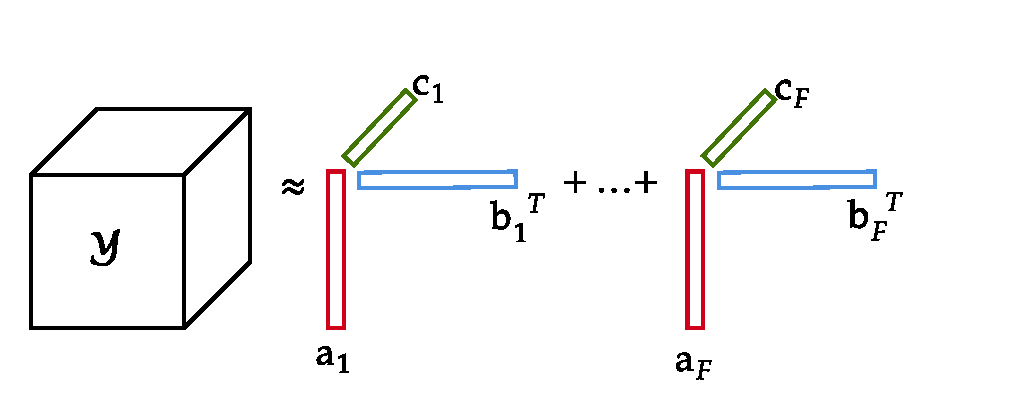
\includegraphics[height=1.5cm]{figures/cp}
\]

\item Tucker: $IR_1+JR_2+KR_3 +R_1R_2 R_3 - R_1^2 - R_2^2 - R_3^2$ 
\[
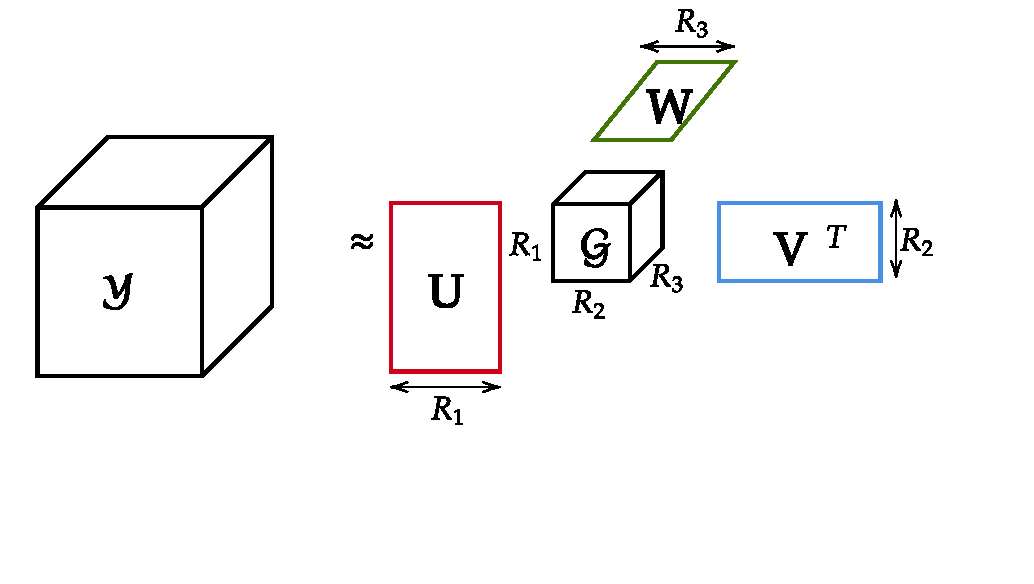
\includegraphics[height=2.5cm]{figures/tucker}
\]
\vspace{-3em}
\end{itemize}

Usages principaux:
\begin{itemize}
\item Tucker: compression (meilleurs algorithmes  )
\item CP: identification (grace à des propriétés d'\textbf{unicité})
\end{itemize}

\end{frame}


%\section{Unicité}
%
%\begin{frame}
%\frametitle{Unicité de la décomposition CP}
%\begin{center}
%
\includegraphics[width=5cm]{figures/keep-calm-and-be-unique-350}
%\end{center}
%\end{frame}
%
%
%\begin{frame}{Cas matriciel}
%\[
%\raisebox{-0.35\height}{\begin{tikzpicture}[scale=0.8]
%\draw(4.7,0.5) node (A) {$\mathbf{M}$};
%\draw(4,0) rectangle (5.4,1);
%
%\draw(5.7,0.5) node (eq) {$=$};
%\draw(6.25,0) rectangle (6.85,1.2); %node {A};
%\draw(6.55,0.6) node (A) {$A$};
%%\draw(5,0.5) node (eq) {\footnotesize$\quad+\,\cdots\,+\quad$};
%\draw(7,0.65) rectangle (8.2,1.2); %node {A};
%\draw(7.6,0.95) node (A) {$B^{T}$};
%
%\draw(8.5,0.5) node (eq) {$=$};
%\draw(8.75,0) rectangle (9.35,1.2); %node {A};
%\draw(9.05,0.6) node (A) {$A$};
%%%\draw(5,0.5) node (eq) {\footnotesize$\quad+\,\cdots\,+\quad$};
%\draw(10.9,0.65) rectangle (12.1,1.2); %node {A};
%\draw(11.5,0.95) node (A) {$B^{T}$};
%
%\draw(9.5,0.65) rectangle (10.05,1.2); %node {A};
%\draw(10.2,0.65) rectangle (10.75,1.2); %node {A};
%
%
%\draw(9.75,0.925) node (A) {\Red{\small $S$}};
%\draw(10.5,0.975) node (A) {\Red{\small $S^{\text{-}1}$}};
%\end{tikzpicture}}
%\]
%indétermination: ordre, échelle, rotation
%
%
%\vspace{1em}
%
%Pas d'unicité sans contraintes (e.g. nonnegativité dans NMF).
%\end{frame}
%
%
%
%\begin{frame}\frametitle{Unicité essentielle}
%
%
%\textbf{Unicité essentielle} : aux indéterminations d'ordre et d'échelle près.
%$$
%[\![\mathbf{A}, \mathbf{B}, \mathbf{C}]\!] = [\![\mathbf{A}\bm{\Pi} \bm{\Delta_A}, \mathbf{B}\bm{\Pi} \bm{\Delta_B}, \mathbf{C}\bm{\Pi} \bm{\Delta_C}]\!]
%$$ 
%avec
%\begin{itemize}
%\item $ \bm{\Pi}$ : matrice de permutation 
%\item $\bm{\Delta_A},\ \bm{\Delta_B}, \ \bm{\Delta_C}$ : matrices diagonales telles que $\bm{\Delta_A} \bm{\Delta_B} \bm{\Delta_C} = \mathbf{I}$
%\end{itemize}
%
%\[
%\updownarrow
%\]
%
%
%Permutation et changement d'échelle de termes de rang 1
%\[
%\Xx = \bfa_1 \circ \bfb_1 \circ \bfc_1 + \cdots+ \bfa_R \circ \bfb_R \circ \bfc_R = \sum\limits_{r=1}^{R} \frac{1}{\alpha_r\beta_r\gamma_r}(\alpha_r\bfa_r) \circ (\beta_r\bfb_r) \circ (\gamma_r\bfc_r) 
%\]
%\end{frame}
%
%\begin{frame}\frametitle{Theorème de Kruskal}
%\textbf{Rang de Kruskal }$k_{\mathbf{A}}$ : valeur maximale de $k$ telle que toute sélection de $k$ colonnes de $\mathbf{A}$ forme une famille libre ($k_{\mathbf{A}} \leq r_{\mathbf{A}} = \text{rang }\mathbf{A}$).
%\\[2ex]
%Remarque : $\text{spark}(\mathbf{A}) = k_{\mathbf{A}}+1$
%\\[2ex]
%\textbf{Exemples} :
%$$
%\mathbf{A}= [ 
%    \mathbf{a}_1  \quad  \mathbf{a}_2  \quad \mathbf{a}_3 \quad \mathbf{a}_4 ]
%$$
%
%$$
%\mathbf{A}= [\mathbf{a}_1 \quad \mathbf{a}_1 \quad \mathbf{a}_3  \quad \mathbf{a}_4]
%$$
%
%$$
%\mathbf{A}= [\mathbf{a}_1 \quad \mathbf{a}_2  \quad \mathbf{a}_1+ \mathbf{a}_2 \quad \mathbf{a}_4]
%$$
%
%\textbf{Condition de Kruskal} : si  $k_{\mathbf{A}},  k_{\mathbf{B}}, k_{\mathbf{C}} \geq 2$ et $k_{\mathbf{A}} + k_{\mathbf{B}} + k_{\mathbf{C}} \geq 2 R +2 $, alors $[\![\mathbf{A}, \mathbf{B}, \mathbf{C}]\!] $ est essentiellement unique $[$Kruskal, 1977$]$.
%\\[2ex]
%Si $k_{\mathbf{A}}=1$, modèle non identifiable
%
%\end{frame}
%
%
%
%\begin{frame}\frametitle{Condition de Kruskal}
%\[
%k_{\mathbf{A}} + k_{\mathbf{B}} + k_{\mathbf{C}} \geq 2 R +2 
%\]
%\begin{itemize}
%\item \textbf{Cas d'une matrice de rang colonne plein} : si $\mathbf{C}$ est de rang colonne plein et que les matrices $\mathbf{A}$ et $\mathbf{B}$ satisfont  1) $k_{\mathbf{A}},  k_{\mathbf{B}}  \geq 2$ et 2)
%$ r_{\mathbf{A}} + k_{\mathbf{B}} \geq  R +2 $ ou $ r_{\mathbf{B}} + k_{\mathbf{A}} \geq  R +2 $ alors  $[\![\mathbf{A}, \mathbf{B}, \mathbf{C}]\!] $ est essentiellement unique $[$Guo, 2011$]$.
%\item Conditions d'identifiabilité partielle $[$Guo et al., 2013$]$ (unicité d'un des facteurs).
%\item
%\textbf{Identifiabilité générique } (tenseur cubique) : si $\mathbf{A}$, $\mathbf{B}$ et $\mathbf{C}$ sont des matrices dont les valeurs sont des réalisations de v.a. à densité absolument continue et dont les dimensions sont telles que $I, \ J , \ K$ alors $[\![\mathbf{A}, \mathbf{B}, \mathbf{C}]\!] $ est essentiellement unique si $R \leq \lceil \frac{I^3}{3I-2}\rceil$  $[$Lickteig, 1986$]$ (extensions pour le cas non-cubique: $[$Chiantini et al., 2015$]$).
%\end{itemize}
%
%\textbf{\color{blue} Matlab (demo 3) }
%\end{frame}


\section{Applications}

\begin{frame}[noframenumbering,plain]{Plan}
\tableofcontents[currentsection]
\end{frame}


\begin{frame}
\frametitle{Exemple jouet}

On considère un tenseur $\Xx$:
\begin{itemize}
	\item[-] 5 capteurs industriels
	\item[-] 50 instants de mesure
	\item[-] 100 fréquence (e.g. imagerie hyperspectrale)
\end{itemize}

\eq{
	\Xx \simeq \sum_{r=1}^R a_r \circ b_r \circ c_r
}

\begin{tcolorbox}
\begin{itemize}
	\item[-] $R$ : modes de fonctionnement du système	
	\item[-] $a_r$ : capteurs sont impliqués, et leur importance
	\item[-] $b_r$ : signature temporelle (quels instants sont concernés) 
	\item[-] $c_r$ : la signature fréquentielle (quelles fréquences sont concernées)
\end{itemize}
\end{tcolorbox}

\end{frame}

\begin{frame}
\frametitle{Exemple en chimiometrie (MEEF)}
\uncover<4>{
\[
\begin{array}{l} 
\text{spectroscopie de fluorescence} \\
\text{matrice d'Emission/Excitation } \\
\end{array}\quad
\begin{array}{c} 
\text{ \Red{rang = \# composants} de mélange} \\
\text{$N$ experimentations, \textcolor{blue}{concentrations différentes}} \\
\end{array}
\]}
\[
\begin{array}{c@{}l}
\text{\uncover<4->{\raisebox{-0.45\height}{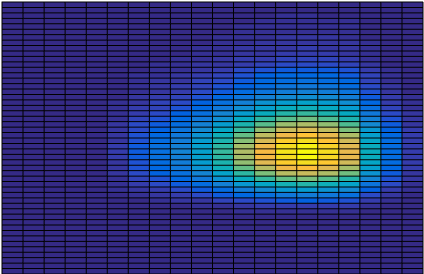
\includegraphics[height=1.2cm]{figures/2dspectrum1}} = }} & 
\raisebox{-0.35\height}{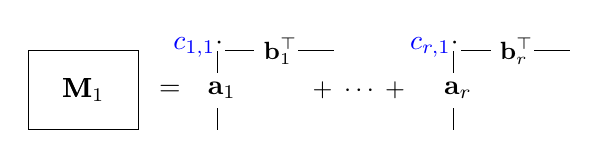
\begin{tikzpicture}
\draw<1>(0,0.5) node (A) {$\mathbf{M}_{\phantom{1}}$};
\draw<2->(0,0.5) node (A) {$\mathbf{M}_1$};
\draw(-0.7,0) rectangle (0.7,1);
\draw(1.1,0.5) node (eq) {${=}$};
\draw(1.7,0) -- (1.7,1);
\draw(1.7,0.5) node[fill=white] (a1) {{ $\bfa_1$}};
\draw(1.8,1) -- (3.18,1);
\draw(2.45,1) node[fill=white] (b1) {{\small $\bfb_1^{\T}\!\!$}};
\draw(3.5,0.5) node () {{\small $+\; \cdots\;+$}};
\draw(4.7,0) -- (4.7,1);
\draw(4.7,0.5) node[fill=white] (a1) {{ $\bfa_r$}};
\draw(4.8,1) -- (6.18,1);
\draw(5.45,1) node[fill=white] (b1) {{\small $\bfb_r^{\T}\!\!$}};

\draw<2->(1.4,1.05) node (eq) {{ $\textcolor{blue}{c_{1,1}}\cdot$}};
\draw<2->(4.4,1.05) node (eq) {{ $\textcolor{blue}{c_{r,1}}\cdot$}};
\end{tikzpicture}} \\
\uncover<4->{\vdots}& \qquad\uncover<2->{\vdots} \\
\text{\uncover<4->{{\raisebox{-0.45\height}{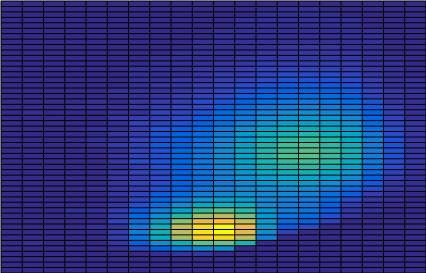
\includegraphics[height=1.2cm]{figures/2dspectrum2}}} = }} & 
\uncover<2->{\raisebox{-0.35\height}{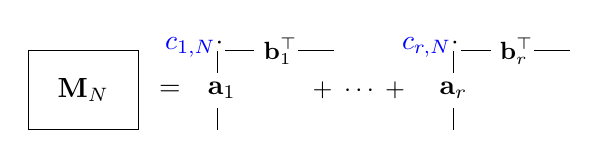
\begin{tikzpicture}
\draw(0,0.5) node (A) {$\mathbf{M}_N$};
\draw(-0.7,0) rectangle (0.7,1);
\draw(1.1,0.5) node (eq) {${=}$};
\draw(1.7,0) -- (1.7,1);
\draw(1.7,0.5) node[fill=white] (a1) {{ $\bfa_1$}};
\draw(1.8,1) -- (3.18,1);
\draw(2.45,1) node[fill=white] (b1) {{\small $\bfb_1^{\T}\!\!$}};
\draw(3.5,0.5) node () {{\small $+\; \cdots\;+$}};
\draw(4.7,0) -- (4.7,1);
\draw(4.7,0.5) node[fill=white] (a1) {{$\bfa_r$}};
\draw(4.8,1) -- (6.18,1);
\draw(5.45,1) node[fill=white] (b1) {{\small $\bfb_r^{\T}\!\!$}};
\draw<2->(1.35,1.05) node (eq) {{ $\textcolor{blue}{c_{1,N}}\cdot$}};
\draw<2->(4.35,1.05) node (eq) {{ $\textcolor{blue}{c_{r,N}}\cdot$}};
\end{tikzpicture}}} \\
& \qquad\qquad\;\; \uncover<3->{\Updownarrow} \\
& \uncover<3->{\!\!\!\!\raisebox{-0.3\height}{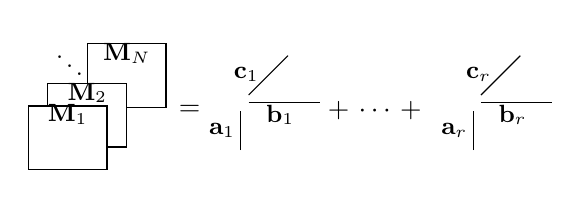
\begin{tikzpicture}
\begin{scope}[scale= 0.5]
%\draw(0.5,0.5) node (A) {$\mathcal{T}$};
%\draw(0,0) rectangle (1,1);
%\draw(0,1) -- (0.5,1.5) -- (1.5,1.5) -- (1.5,0.5) --(1,0);
%\draw(1,1) -- (1.5,1.5);
\draw[fill=white](-0.5,0.88) rectangle (1.5,2.5);
\draw[fill=white](-1.5,-0.12) rectangle (0.5,1.5);
%\draw[fill=white](-0.75,-0.75) rectangle (1.25,1.25);
\draw[fill=white](-2,-0.7) rectangle (0,0.92);
\draw(-1,0.7) node (A) {\small $\bfM_1$};
\draw(-0.5,1.25) node (B) {\small $\bfM_2$};
\draw(0.5,2.25) node (C) {\small $\bfM_N$};
\draw(-0.95,2.15) node (D) {\small $\ddots$};



\draw(2.1,0.8) node (eq) {$=$};
\draw(6.8,0.8) node (eq) {$\quad+\,\cdots\,+\quad$};
\end{scope}

\begin{scope}[scale= 0.5,xshift=1.4cm]
\draw(2,-0.2) -- (2,0.8);
\draw(2.1,0.3) node[anchor=east] (s21) {\small {$\bfa_1$}};
\draw(2.2,1) -- (4,1);
\draw(3.0,1.2) node[anchor=north] (s22) {\small {$\bfb_1$}};
\draw(2.2,1.2) -- (3.2,2.2);
\draw(2.7,1.3) node[anchor=south east] (s23) {\small{$\bfc_1$}};
\end{scope}

\begin{scope}[scale= 0.5,xshift=7.3cm]
\draw(2,-0.2) -- (2,0.8);
\draw(2.1,0.3) node[anchor=east] (s21) {\small {$\bfa_r$}};
\draw(2.2,1) -- (4,1);
\draw(3.0,1.2) node[anchor=north] (s22) {\small {$\bfb_r$}};
\draw(2.2,1.2) -- (3.2,2.2);
\draw(2.7,1.3) node[anchor=south east] (s23) {\small {$\bfc_r$}};
%\draw(1.9,1) node (g1) {\textcolor{red}{\small $c_r$}};
\end{scope}
\end{tikzpicture}}}\\
\end{array}
\]
\end{frame}

\begin{frame}{Exemple: classification d'images}
\textbf{Réseau convolutionnnel}
\[
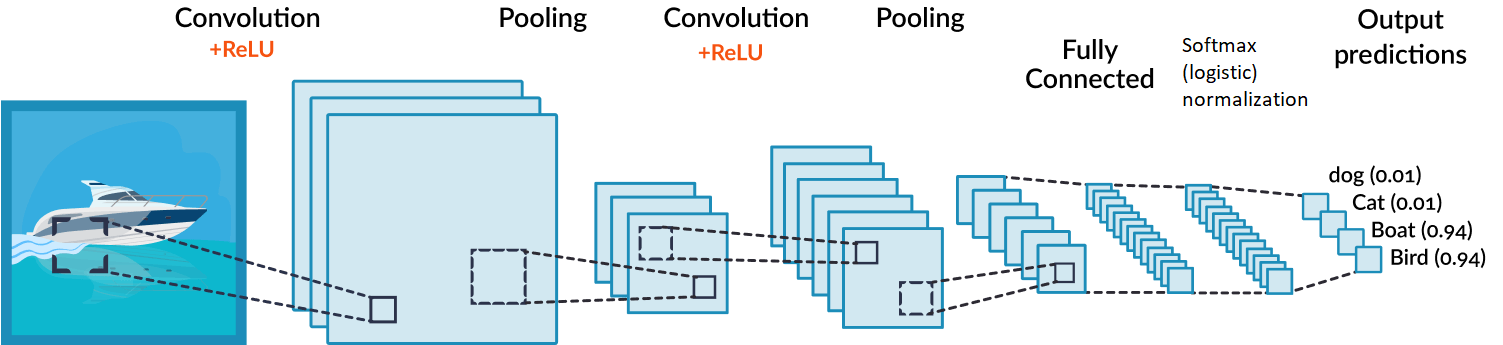
\includegraphics[height=2.5cm]{figures/convnet.png}
\]

\begin{itemize}
\item Inconvenient: cout important de stockage
\end{itemize}

\end{frame}



\begin{frame}{Convolutional layers}
\[
\raisebox{-0.5\height}{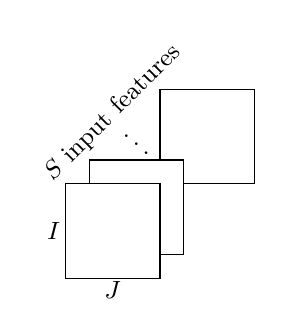
\begin{tikzpicture}
\begin{scope}[scale=0.6]
\draw[fill=white](1,1) rectangle (3,3);
\draw[fill=white](-0.5,-0.5) rectangle (1.5,1.5);
\draw[fill=white](-1,-1) rectangle (1,1);

\draw(0,0) node (A) {$\Uu$};
\draw(0.5,1.25) node (B) {};
\draw(2,2.75) node (C) {};
\draw(0.5,2) node (D) {\small $\ddots$};

\draw(0,-1.25) node (D) {\small $J$};
\draw(-1.25,0) node (D) {\small $I$};
\draw(0,2.5) node[rotate=45] (D) {\small $S$ input features};
\end{scope}
\end{tikzpicture}}
\quad
\xrightarrow{\substack{\text{convolution avec $T$}\\ \text{$(d\times d\times S)$ filtres 2D}} }
\quad
\raisebox{-0.5\height}{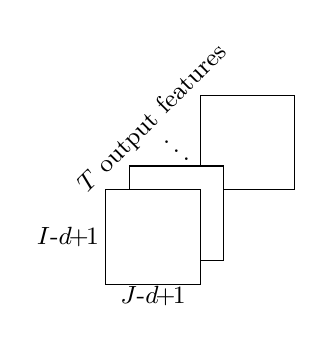
\begin{tikzpicture}
\begin{scope}[scale=0.6]
\draw[fill=white](1,1) rectangle (3,3);
\draw[fill=white](-0.5,-0.5) rectangle (1.5,1.5);
\draw[fill=white](-1,-1) rectangle (1,1);

\draw(0,0) node (A) {$\Vv$};
\draw(0.5,1.25) node (B) {};
\draw(2,2.75) node (C) {};
\draw(0.5,2) node (D) {\small $\ddots$};

\draw(0,-1.25) node (D) {\small $J\text{-}d\!\!+\!\!1$};
\draw(-1.8,0) node (D) {\small $I\text{-}d\!\!+\!\!1$};
\draw(0,2.5) node[rotate=45] (D) {\small $T$ output features};
\end{scope}
\end{tikzpicture}}
\]
\begin{align*}
\mathcal{V}(x,y,t) &= g\Big( \sum\limits_{i=x-d+1}^{x}\sum\limits_{j=y-d+1}^{y} \sum\limits_{s=1}^{S} \mathcal{K}(i-x+d, j-y+d,s,t) \mathcal{U}(i,j,s) \\
& + b(x,y,t)\Big)
\end{align*}
défini par  tensor $4D$  $\Kk \in \RR^{d\times d \times S\times T}$

\vspace{1em}

$\Rightarrow$ compression par décomposition CP


\end{frame}

\begin{frame}{Approximations tensorielles pour la compression de réseaux de neurones}
\emph{\small (Lebedev et al., 2015)}
\[
\mathcal{K} \approx\sum\limits_{r=1}^{R} \bfa_r \circ \bfb_r \circ \bfc_r \circ \bfd_r , 
\]
\[
\!\!\!\! \begin{array}{@{}ccc@{}}
\text{full convolution} & & \text{sequence of 1D convolutions} \\ 
\raisebox{-0.5\height}{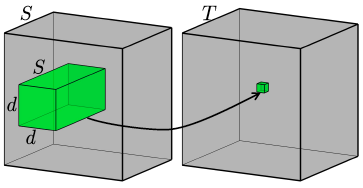
\includegraphics[height=1.6cm]{figures/conv_full.png}} &\to& \raisebox{-0.5\height}{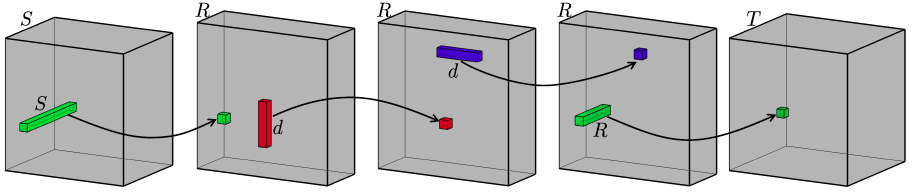
\includegraphics[height=1.6cm]{figures/conv_cpd.png}}
\end{array}
\]


\end{frame}


\begin{frame}
\frametitle{Conclusion}

\begin{itemize}[label=\tiny$\blacksquare$]
	\item Les données se présentent très généralement sous forme matricielles/tensorielles
	\item Nécessité de savoir manipuler ces structures
	\item Il est important d'avoir des méthodes d'approximation/simplification de ces données. Cela passe souvent par des algoithmes de décompositions ou factorisations
	\item Les propriétés mathématiques des décompositions (existence, unicité, etc..) influent sur la complexité du problème.
\end{itemize}
\end{frame}





%\bibliographystyle{apalike}
%\printbibliography
%\bibliography{/export/home/pcatala/Workspace/build/biblio}

\end{document}
